% SETUP
\documentclass[11pt]{article}
\linespread{1.25}
\usepackage[utf8]{inputenc}
\usepackage{graphicx, amsmath, array, graphics, amssymb, epsfig, psfrag, geometry, alltt, subfiles, blindtext, enumitem,float,pdfpages}
\DeclareMathOperator{\sinc}{sinc}
\usepackage[export]{adjustbox}
\usepackage{fancyhdr}
\usepackage{array}
\usepackage{hyperref}
%%%%%%%%%%%%%%  code listing
\usepackage{listings}
\usepackage{color} %red, green, blue, yellow, cyan, magenta, black, white
\definecolor{mygreen}{RGB}{2,94,33} % color values Red, Green, Blue
\definecolor{mylilas}{RGB}{170,55,241}

\lstset{language=Matlab,%
    %basicstyle=\color{red},
    breaklines=true,%
    morekeywords={matlab2tikz},
    keywordstyle=\color{blue},%
    morekeywords=[2]{1}, keywordstyle=[2]{\color{black}},
    identifierstyle=\color{black},%
    stringstyle=\color{mylilas},
    commentstyle=\color{mygreen},%
    showstringspaces=false,%without this there will be a symbol in the places where there is a space
    numbers=left,%
    numberstyle={\tiny \color{black}},% size of the numbers
    numbersep=9pt, % this defines how far the numbers are from the text
    emph=[1]{for,end,break},emphstyle=[1]\color{black}, %some words to emphasise
    %emph=[2]{word1,word2}, emphstyle=[2]{style},    
}
%%%%%%%%%%%%%%%%


\geometry{a4paper, top = 20mm, bottom = 20mm, left = 15mm, right = 15mm}

% Headers
\pagestyle{fancy}
\fancyhf{}
\chead{ELEN90057 Communication Systems - Workshop 1 Report}
\cfoot{\thepage}

\begin{document}
% Title

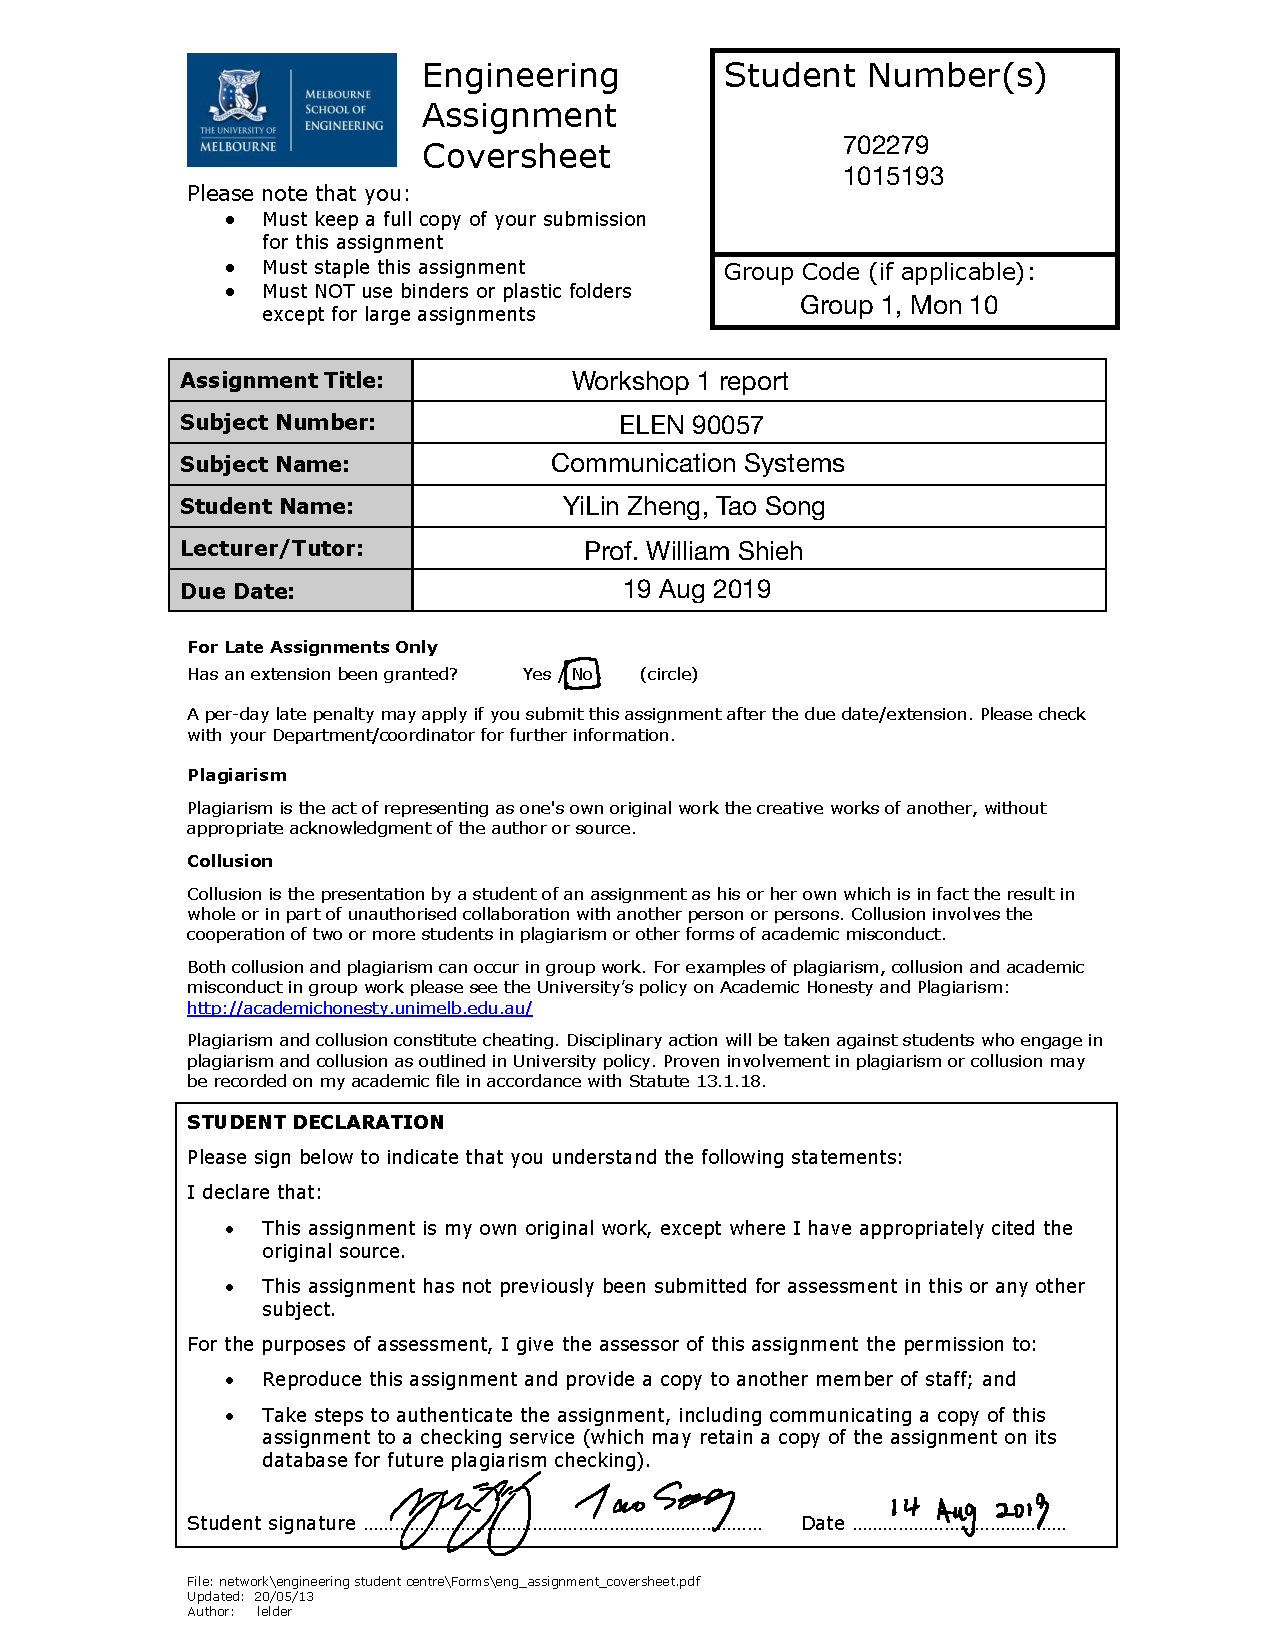
\includepdf{coverpage.pdf}

\newpage

\begin{center}
\textbf{\Large{Workshop 1}}\\
Group 1: Tao Song [1015193], YiLin Inez Zheng [702279], \\
Workshop: Monday 10:00am - 12:00pm (Shalanika, Bigi), Due: 19/08/19  
\end{center}

%%%%%%%%%%%%% BEGIN INPUT SIGNAL %%%%%%%%%%%%%%%%%
\section{Input Signal [8 marks]}
\begin{enumerate}[label=(\alph*)]
    \item %a
    In a complex Fourier series, $x(t)$ is the following,
    \begin{align*}
        x(t) &= \sum_{n = -\infty}^{\infty}x_n e^{j \frac{2\pi}{T_0} nt}\\
        x_n &= \frac{1}{T_0} \int^{\frac{T_0}{2}}_{-\frac{T_0}{2}} x(t) e^{-j \frac{2\pi}{T_0} nt} dt \\
        &= \frac{1}{T_0} \int^{\frac{\tau}{2}}_{-\frac{\tau}{2}} e^{-j \frac{2\pi}{T_0} nt} dt\\
        &= \frac{1}{T_0} \cdot -\frac{1}{j\frac{2\pi}{T_0}n} e^{-j \frac{2\pi}{T_0} nt} \Biggr|_{-\frac{\tau}{2}}^{\frac{\tau}{2}}\\
        &= -\frac{1}{j2\pi n} \Big(
        e^{-j \frac{2\pi}{T_0}n\frac{\tau}{2}} 
        -e^{j \frac{2\pi}{T_0}n\frac{\tau}{2}}\Big)\\
        &= \frac{1}{j2\pi n} \cdot 2j\sin\Big(\frac{2\pi}{T_0}n\frac{\tau}{2}\Big)\\
        \Rightarrow x_n &= \underline{\frac{\tau}{T_0}\sinc \Big(\frac{\tau}{T_0}n\Big)} 
    \end{align*}
    Therefore,
    \begin{align*}
        x(t) &= \sum_{n = \infty}^{\infty} \frac{\tau}{T_0}\sinc \Big(\frac{\tau}{T_0}n\Big) e^{j \frac{2\pi}{T_0} nt}
    \end{align*}
    Now, $X(f)$, the Fourier transform of $x(t)$ at ordinary frequency $f$, by principle of duality,
    \begin{align*}
        e^{j \frac{2\pi}{T_0} nt} &\leftrightharpoons \delta(f - \frac{2\pi}{T_0} n \cdot \frac{1}{2\pi}) = \delta(f - \frac{n}{T_0})\\
        x(t) &\leftrightharpoons X(f)\\
        \sum_{n = -\infty}^{\infty}x_n e^{j \frac{2\pi}{T_0} nt} 
        &\leftrightharpoons \sum_{n = -\infty}^{\infty} \frac{\tau}{T_0}\sinc \Big(\frac{\tau}{T_0}n\Big)\delta(f - \frac{n}{T_0})\\
        \Rightarrow X(f) &= \underline{\sum_{n = -\infty}^{\infty} \frac{\tau}{T_0}\sinc \Big(\frac{\tau}{T_0}n\Big)\delta(f - \frac{n}{T_0})}
    \end{align*}
    
    \item %b 
    Finding the power expression for $x(t)$, considering one period $T_0$,
    \begin{align*}
        P(t) &= \frac{1}{T_0} \int^{\frac{T_0}{2}}_{-\frac{T_0}{2}} |x(t)|^2 dt\\
        &= \frac{1}{T_0} \int^{\frac{\tau}{2}}_{-\frac{\tau}{2}} 1 dt = \frac{1}{T_0} \Big(\frac{\tau}{2} - -\frac{\tau}{2}\Big) = \frac{\tau}{T_0}\\
        \Rightarrow P(t) &= \underline{\frac{\tau}{T_0}} 
    \end{align*}
    For the given values $T_0 = 1$ and $\tau=0.4$, $P(t)=0.4$.\\
    
    To calculate the spread of 98\% power across the Dirac impulses in the Fourier transform $X(f)$, we sum the terms in its spectral power.
    \begin{align*}
        P &= \sum_{n = -\infty}^{\infty} |x_n|^2\\
        &= \sum_{n = -\infty}^{\infty}\Biggr|\frac{\tau}{T_0}\sinc \Big(\frac{\tau}{T_0}n\Big)\Biggr|^2
    \end{align*}
    with the given $T_0$ and $\tau$ values,
    \begin{align*}
        P &= \sum_{n = -\infty}^{\infty}\Big|0.4\sinc(0.4n)\Big|^2 \geq 0.4 \cdot 0.98 = 0.392
    \end{align*}
    From MATLAB, we calculated the bandwidth, $W$ to be 13Hz.
    
    \begin{figure}[h]
        \centering
        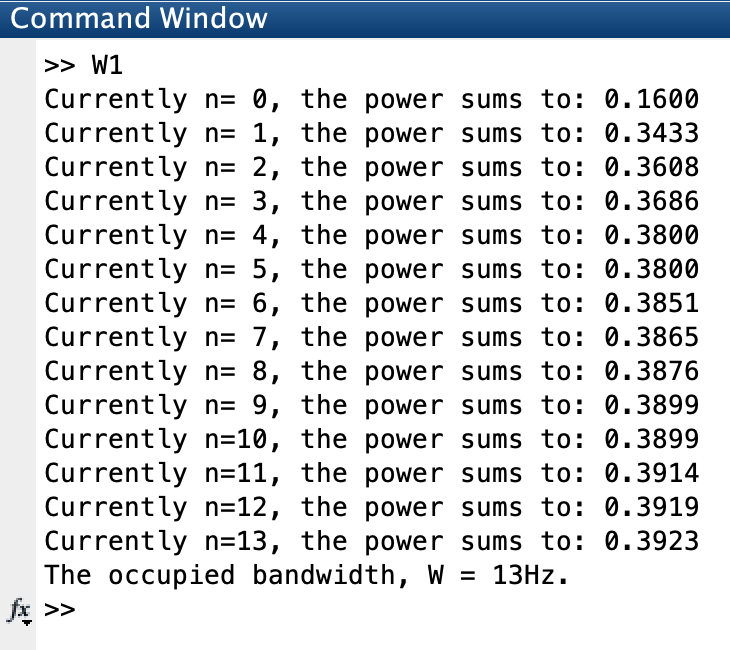
\includegraphics[scale=0.6]{W1Q1b.png}
        \caption{Output in MATLAB - See code in Appendix}
        \label{fig:W1Q1b}
    \end{figure}{}
    \textit{* Note}: From the iterated values we can see that $W=12Hz$ yields a rather accurate power summation to the spectrum 98\% power of 0.32. However, reading the fine print on our lab sheets that say strictly $W$ is defined at the 99\% occupation, we conclude that $W=13Hz$ could truly represent the occupied bandwidth by being just over the 98\% power threshold value.
\end{enumerate}

%%%%%%%%%%%% BEGIN CHANNEL EQUALISATION SECTION %%%%%%%%%%%%%%%%
\section{Channel Equalisation [10 marks]}
\begin{enumerate}[label=(\alph*)]
\item %a
To find frequency response $H(f)$, we first take the Laplace transformation of $RC\frac{d}{dt}y(t)+y(t)=x(t)$, 
\begin{align*}
        RCsY(s)+Y(s)&=X(s)\\
        (1+RCs)Y(s)&=X(s) \\
        H(s)=\dfrac{Y(s)}{X(s)}&=\dfrac{1}{1+RCs}
\end{align*}
From here, frequency response $H(f)$ can be expressed by letting $s=j2\pi f$,
\begin{align*}
        \Rightarrow H(f)=\underline{\dfrac{1}{1+j2\pi f RC}}
\end{align*}
In terms of 3dB bandwidth $B$, the power magnitude at the 3dB frequency $f_c$ is $\frac{1}{2}$. For the low-pass filter, the upper band of bandwidth $B$ is the value of $f_c$ while lower band is 0 Hz (in the spectrum, both the positive and negative side should be symmetric).
\begin{align*}
        |H(f_c)|^2 &=\Big(\sqrt{H(f_c)\times H^*(f_c)} \Big)^2\\ 
        &=\dfrac{1}{(1+j2\pi f_c RC)(1-j2\pi f_c RC)}\\
        &=\dfrac{1}{1+(2\pi f_c RC)^2} = \frac{1}{2}\\
        \Rightarrow B = f_c &=\underline{\dfrac{1}{2\pi RC}}
\end{align*}

\item %b
The signal $x(t)$ will display transmission distortions when passed through the channel. As shown in the MATLAB plots in Figure \ref{fig:q2b}, there are both amplitude and phase distortions. The frequency domain output $Y(f)$ has significant distortions outside of the passband range of $\pm0.5$Hz.\\
\textit{Amplitude distortion} is caused by the low pass filter magnitude $|H(f)| = \frac{1}{\sqrt{1 + (2\pi fRC)^2}}$ not having a constant response.\\
\textit{Delay distortion} is due to the low pass filter argument $\arg H(f) = \arctan(2\pi fRC) $ not having a negative linear phase shift (delay).\\
\textit{Time-domain waveform of $y(t)$ can be found in Figure \ref{fig:q2e} in Q2e).}

\begin{figure}[H]
    \centering
    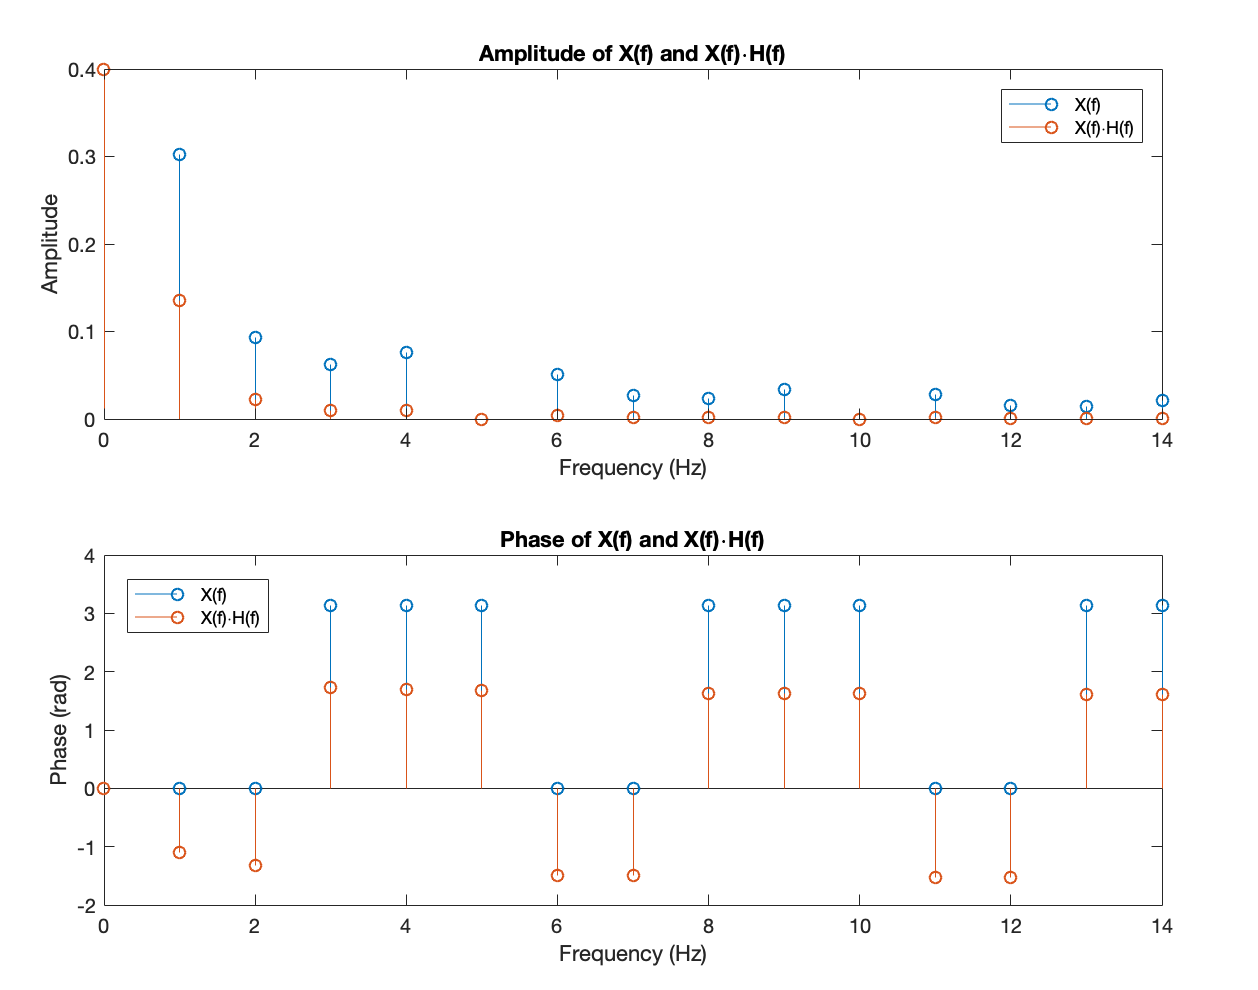
\includegraphics[scale = 0.5]{W1Q2b.png}
    \caption{\label{fig:q2b}Discrete plot of $X(f)$'s angle and magnitude before and after the low pass filter $H(f)$}
\end{figure}

\textit{* Note}: Just to specify how to find the expression of $Y(f)$ and $y(t)$. The output waveform from the low-pass filter can be found by,  
\begin{align*}
        Y(f)&= H(f)X(f)\\
        &= \dfrac{1}{1+j2\pi fRC} \sum_{n = -\infty}^{\infty} \frac{\tau}{T_0}\sinc \Big(\frac{\tau}{T_0}n\Big)\delta(f - \frac{n}{T_0})
\end{align*}
Previous conclusions revealed that, $B = f_c =\frac{1}{2\pi RC}=0.5$Hz, which means $RC= \frac{1}{\pi}$.\\
Therefore, $Y(f)$ can be expressed by the following and to find $y(t)$, simply take the inverse Fourier transform of $Y(f)$.
\begin{align*}
        Y(f)&= \sum_{n = -\infty}^{\infty} \dfrac{1}{1+j2f}  \frac{\tau}{T_0}\sinc \Big(\frac{\tau}{T_0}n\Big)\delta(f - \frac{n}{T_0}) \\
        &= \sum_{n = -\infty}^{\infty} \dfrac{\tau}{1+j2n} \sinc \Big(\frac{\tau}{T_0}n\Big)
\end{align*}

\item %c 
An ideal equaliser is capable to maintain a constant magnitude gain and linear phase shift (constant time delay $t_d$). Our ideal output $V(f)$ can be created through a time and amplitude shift, 
\begin{align*}
    V(f)=Ke^{-j2 \pi f t_d}X(f)
\end{align*}
where,
$Ke^{-j2 \pi f t_d}=H(f)H_{eq}(f)$.

The frequency response $H_{eq}(f)$ of an ideal equaliser can be then expressed as,
\begin{align*}
    H_{eq}(f)=\dfrac{Ke^{-j2 \pi f t_d}}{H(f)}=Ke^{-j2 \pi f t_d}H^{-1}(f)
\end{align*}
substituting $H^{-1}(f)=1+j2\pi f RC$, 
\begin{align*}
   H_{eq}(f)=  Ke^{-j2 \pi f t_d}(1+j2\pi f RC)
\end{align*}
where $K = |H(f)| = \frac{1}{\sqrt{1 + (2\pi f RC)^2}}$ and $t_d = -\frac{arg H(f)}{2\pi f} = -\frac{\arctan(2\pi fRC)}{2\pi f}$ are constants.\\

In addition, $RC=\frac{1}{\pi}$. Therefore, the frequency response can be further simplified as,
\begin{align*}
  \Rightarrow H_{eq}(f)=  \underline{Ke^{-j2 \pi f t_d}(1+j2f)}
\end{align*}

\item There are two ways to solve this question,
\begin{enumerate}
\item[1.] Convolution of the impulse response of $h_{eq}(t)$ and $y(t)$
\item[2.] Inverse Fourier transform of $V(f)$.
\end{enumerate}
The first way: To find $h_{eq}(t)$, we can take the inverse Fourier transform of $H_{eq}(f)$,
\begin{align*}
    H_{eq}(f)&=  Ke^{-j2 \pi f t_d}(1+j2f)\\
    H_{eq}(\omega)&=Ke^{-j\omega t_d}(1+j\dfrac{\omega}{\pi})\\
    h_{eq}(t)&=\dfrac{K}{2\pi} \int_{-\pi}^{\pi} e^{-j\omega t_d} (1+j\dfrac{\omega}{\pi})d\omega \\
\end{align*}
Taking integration by parts,
\begin{align*}
    h_{eq}(t)&=\dfrac{K}{2\pi} ([(1+j\dfrac{\omega}{\pi})\dfrac{e^{-j\omega t_d}}{-jt_d}]_{-\pi}^{\pi}  +\int_{-\pi}^{\pi}\dfrac{ e^{-j\omega t_d}}{t_d\pi} d\omega)\\
    &=\dfrac{K}{2\pi} [(1+j)\dfrac{ e^{-j\pi t_d}}{-jt_d}-(1-j)\dfrac{ e^{j\pi t_d}}{-jt_d}+[\dfrac{e^{-j\omega t_d}}{-jt_d}\dfrac{1}{t_d\pi}]_{-\pi}^{\pi}]\\
    &=\dfrac{K}{2\pi} [(1+j)\dfrac{ e^{-j\pi t_d}}{-jt_d}-(1-j)\dfrac{ e^{j\pi t_d}}{-jt_d}+\dfrac{1}{t_d \pi}(\dfrac{e^{-j\pi t_d}-e^{j\pi t_d}}{-j t_d})]\\
    &= \frac{K}{2\pi}(\dfrac{e^{-j\pi t_d}+je^{-j\pi t_d}-e^{j\pi t_d}+je^{j\pi t_d}+\dfrac{e^{-j\pi t_d}-e^{j\pi t_d}}{t_d \pi}}{-j t_d}) \\
    &= \frac{K}{2\pi}(\dfrac{e^{-j\pi t_d}+je^{-j\pi t_d}-e^{j\pi t_d}+je^{j\pi t_d}+\dfrac{-j2sin(\pi t_d)}{t_d \pi}}{-j t_d}) \\
    &=\frac{K}{\pi}(\dfrac{sin(\pi t_d)-cos(\pi t_d)+\dfrac{sin(\pi t_d)}{t_d \pi}}{t_d}) \\
    &=K\Big (\dfrac{sin(\pi t_d)-cos(\pi t_d)}{\pi t_d}+\dfrac{sin(\pi t_d)}{\pi ^2  t_d^2}\Big)
\end{align*}    
$V(f)=H_{eq}(f)Y(f)$ in frequency domain, in time domain we have,
\begin{align*}
    v(t)&=h_{eq}(t)*y(t)\\
    \Rightarrow v(t)&=\underline{h_{eq}(t)*y(t)=K\Big (\dfrac{sin(\pi t_d)-cos(\pi t_d)}{\pi t_d}+\dfrac{sin(\pi t_d)}{\pi ^2  t_d^2}\Big) * y(t)}
\end{align*}
Alternatively,
\begin{align*}
V(f)&=H_{eq}(f)Y(f)\\
&=Ke^{-j2\pi f t_d}(1+j2f)Y(f)\\
&=Ke^{-j2\pi f t_d}Y(f)+j2fKe^{-j2\pi f t_d}Y(f)
\end{align*}
taking inverse Fourier transform, we will have,
\begin{align*}
\Rightarrow \underline{v(t)=Ky(t-t_d)+\dfrac{K}{\pi}\dfrac{d}{dt}y(t-t_d)}
\end{align*}
\textit{* Note}: We used the ideal equaliser $H_{eq}(f)$ we obtained in Q2c) with $RC = \frac{1}{\pi}$ for the derivations this section.
A general time domain expression for $v(t)$ in terms of $y(t)$ through a RC low pass filter would be, $v(t)=Ky(t-t_d)+KRC\dfrac{d}{dt}y(t-t_d)$.\\

\item %e
We passed through a pulse signal as $x(t)$, which produced the unequalised output $y(t)$ (implementing the RC circuit time domain expression, which is the same as passing through $H(f)$ from Q2a) in the frequency domain). We used the unit delay block for $t_d$ and a $K=1$ gain block in Simulink to model the equaliser in the time domain and produced $v(t)$ as expressed in Q2d).\\
    \begin{figure}[H]
        \centering
        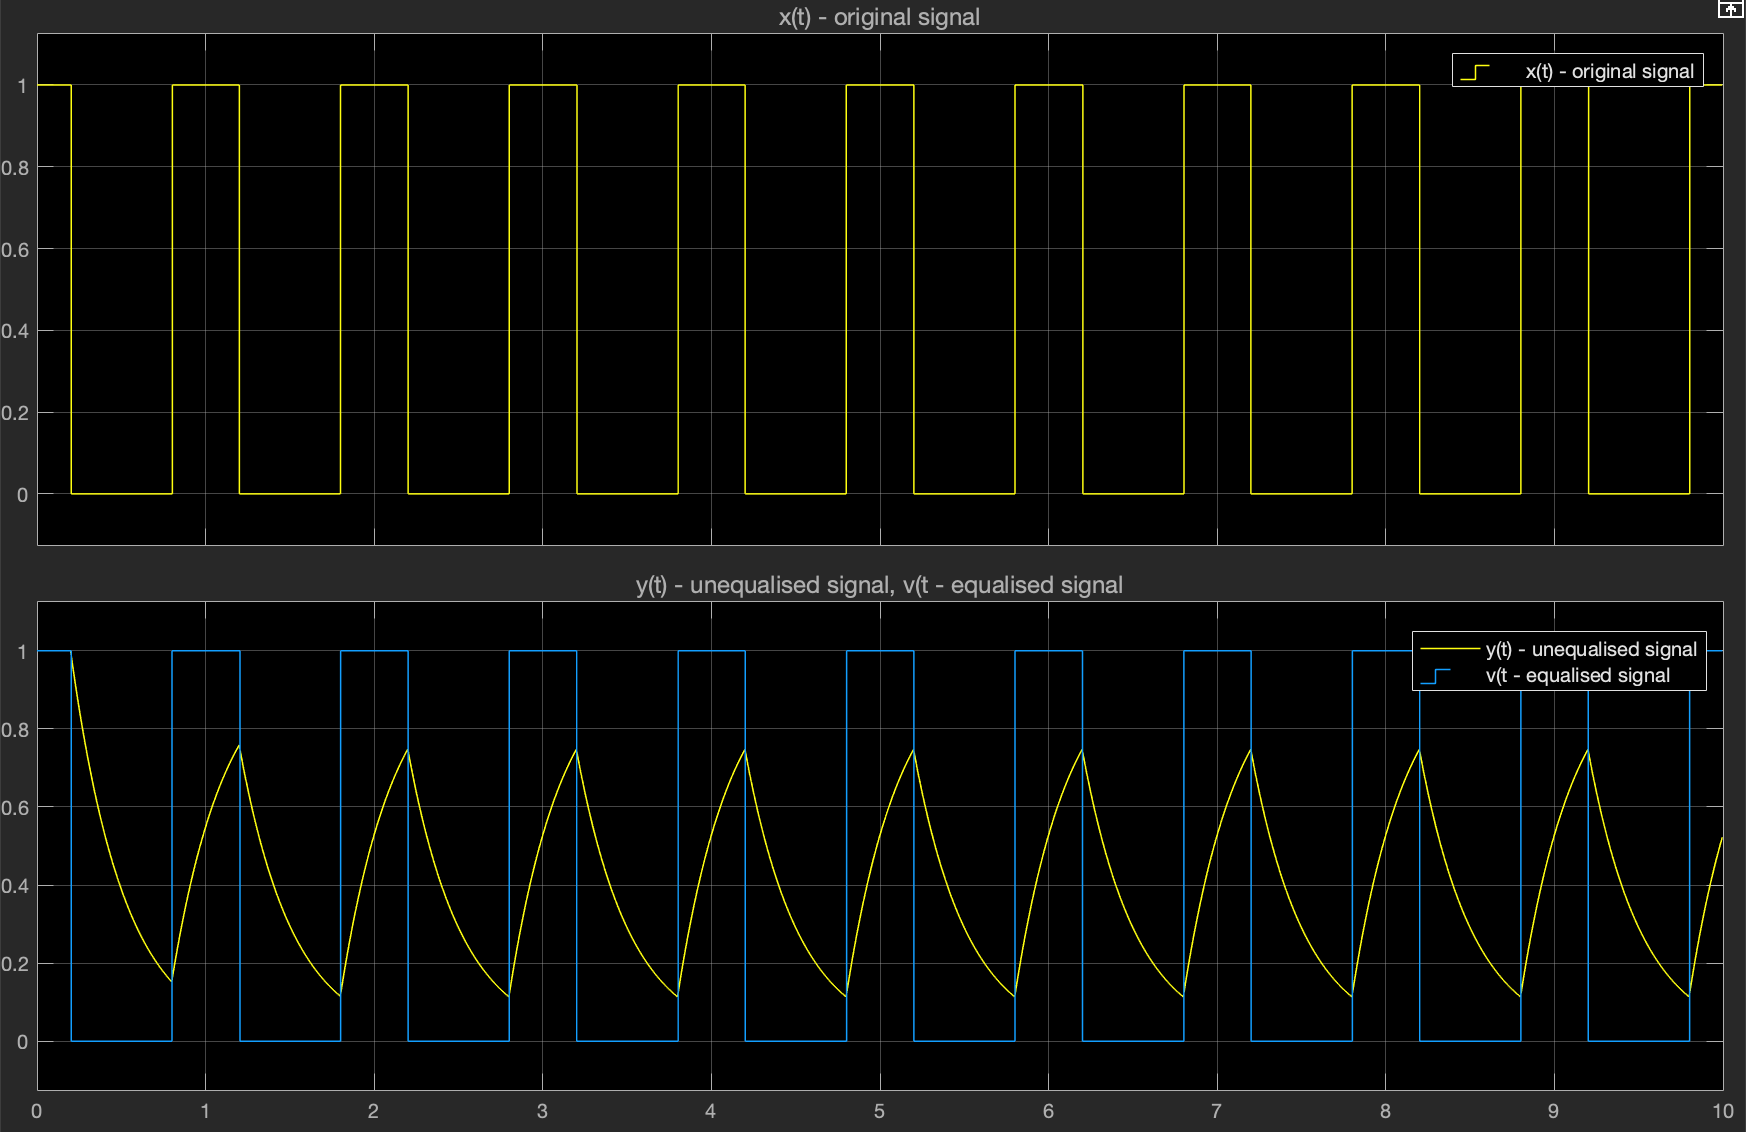
\includegraphics[scale=0.5]{W1Q2e.png}
        \caption{\label{fig:q2e}Original input $x(t)$, unequalized output $y(t)$ and equalized output $v(t)$ signals through a low-pass filter in time domain}
    \end{figure}
    \begin{figure}[ht!]
    \centering
        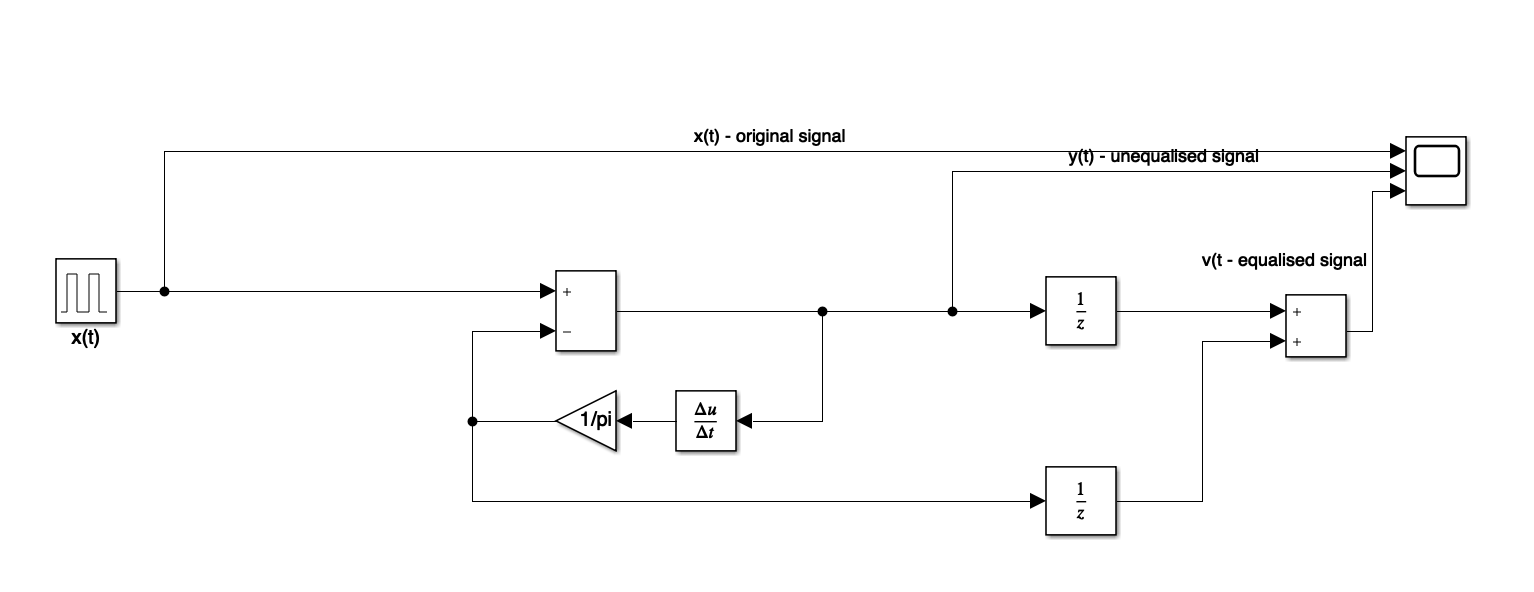
\includegraphics[scale=0.5]{W1Q2e_SimuLink.png}
        \caption{\label{fig:q2eblocks}Simulink model to generate the low pass filter and equaliser}
    \end{figure}
 
As seen, the input signal $x(t)$ was distorted after passing through the low-pass filter. There are some observations from Figure \ref{fig:q2e}: 
\begin{itemize}
  \item The signal shape was changed, which is closer to a low frequency sinusoidal waveform. 
  \item High frequency components, which mainly form the right angles for the rectangular pulse, were disappeared.
\end{itemize}
After the distorted signal passed through the ideal equaliser, the output signal matched the original signal $x(t)$, indicating a distortion-less transmission. For this perfect outcome we set our simulation solver's additional parameter as "Max Step Size = 1e-3".
\end{enumerate}

%%%%%%%%%%%% BEGIN TRANSVERSAL FILTER SECTION %%%%%%%%%%%%%%%%
\section{Transversal Filter [12 marks]}
\begin{enumerate}[label=(\alph*)]
\item %a
As discovered in Question 2 when building the equaliser, $H^{-1}(f) = 1 + j2\pi fRC$. In this problem, $\Delta=\dfrac{1}{2W}$. Fourier series coefficient $d_n$ can be expressed as, %Expressing in Fourier Series,
%\begin{align*}
%    H^{-1}(f) = \sum^{\infty}_{n = -\infty} d_n e^{j2\pi n\Delta f}
%\end{align*}
\begin{align*}
    d_n &=\dfrac{1}{2W} \int^{W}_{-W} (1 + j2\pi fRC) e^{-j2\pi \dfrac{n}{2W} f} df \\
    &=\Delta \int^{\frac{0.5}{\Delta}}_{-\frac{0.5}{\Delta}} (1 + j2\pi fRC)e^{-j2\pi n \Delta f} df \\
    &= \Delta \int^{\frac{1}{2\Delta}}_{-\frac{1}{2\Delta}} (e^{-j2\pi n \Delta f} + j2\pi fRC e^{-j2\pi n \Delta f}) df \\
    &= \Delta \Biggr(\Biggr[\frac{e^{-j2\pi n \Delta f}}{-j2\pi n \Delta}\Biggr]^{\frac{1}{2\Delta}}_{-\frac{1}{2\Delta}}
    + j2\pi RC\Big(\Big [f \cdot \frac{e^{-j2\pi n \Delta f}}{-j2\pi n \Delta} \Big]^{\frac{1}{2\Delta}}_{-\frac{1}{2\Delta}} - \int^{\frac{1}{2\Delta}}_{-\frac{1}{2\Delta}} \frac{e^{-j2\pi n \Delta f} }{-j2\pi n \Delta }df\Big)
    \Biggr)\\
    &= \Delta \Biggr( \frac{sin(\pi n)}{\pi n \Delta}  + \frac{j2\pi RC cos(\pi n)}{-j2\pi n\Delta^2} - \frac{jRC sin(\pi n)}{\pi n^2 \Delta^2} \Biggr)  \\
    &=  \frac{sin(\pi n)}{\pi n }  + \frac{ RC cos(\pi n)}{- n\Delta} - \frac{jRC sin(\pi n)}{\pi n^2 \Delta}   \\
    &= \frac{ -RC }{ n\Delta}(-1)^n
\end{align*}
for $n=0$,$d_n$ can be obtained by, 
\begin{align*}
d_n &=\dfrac{1}{2W} \int^{W}_{-W} (1 + j2\pi fRC) e^{-j2\pi \dfrac{0}{2W} f} df \\
&=\dfrac{1}{2W} \int^{W}_{-W} (1 + j2\pi fRC) df\\
&=\dfrac{1}{2W} \Big [f+j\pi RC f^2 \Big] _{-W}^{W} \\
&= 1
\end{align*}
in conclusion, $d_n$ can be expressed as,
\begin{align*}
\Rightarrow \underline{d_n=\left\{
             \begin{array}{lr}
             1, & n=0\\
             \frac{ -RC }{ n\Delta}(-1)^n & elsewhere
             \end{array}
\right. }
\end{align*}
\item %b
%By reading the transversal filter graph, 
%\begin{align*}
%    v(t) = y(t)c_0+y(t-\Delta)c_1+y(t-2\Delta)c_2+......+ y(t-2M\Delta)c_{2M}   
%\end{align*}
%in frequency domain,
%\begin{align*}
%    V(f) = Y(f)c_0+Y(f)e^{-j\omega\Delta}c_1+Y(f)e^{-j\omega 2\Delta}c_2+......+ Y(f)e^{-j\omega 2M\Delta}c_{2M}   
%\end{align*}
%therefore, the transfer function can be found as,
%\begin{align*}
%    H_{tf}(f)=\dfrac{V(f)}{Y(f)} &= c_0+e^{-j\omega\Delta}c_1+e^{-j\omega 2\Delta}c_2+......+ e^{-j\omega 2M\Delta}c_{2M} \\
%    &= \sum _{m=0}^{m=2M} c_m e^{-j\omega m\Delta} , c_m=d_m
%\end{align*}
To have a distortion-less signal, it must maintain that,
\begin{align*}
    H_{tf}(f)H(f)=Ke^{-j 2 \pi f M \Delta} \\
    H_{tf}(f)=H^{-1}(f)Ke^{-j2 \pi f M \Delta}
\end{align*}
we let $K=1$ to simplify the analysis,
\begin{align*}
    H^{-1}(f) &= \sum ^{M}_{m=-M} d_m e^{j2\pi fm \Delta}\\
    &=e^{j2\pi fM \Delta} \sum ^{M}_{m=-M} d_m e^{j2\pi f(m-M) \Delta}\\
\end{align*}
let $n=M-m$, i.e., $m=M-n$, therefore,
\begin{align*}
H^{-1}(f) &=e^{j2\pi fM \Delta} \sum ^{2M}_{n=0} d_{M-n} e^{-j2\pi fn \Delta}\\
&= H_{tf}(f)e^{j 2\pi f M \Delta}
\end{align*}
this gives,
\begin{align*}
H_{tf}(f)=\sum ^{2M}_{n=0} d_{M-n} e^{-j2\pi fn \Delta}
\end{align*}
The system output $V(f)$ is determined by,
\begin{align*}
V(f)=X(f)H(f)H_{tf}(f)=X(f)Ke^{-j2 \pi f M \Delta}
\end{align*}
Take inverse Fourier transfer, in time domain, the output will be,
\begin{align*}
\Rightarrow \underline{ v(t)=Kx(t-M \Delta) }
\end{align*}
That is, the output from the filter in time domain will be: the input signal boosted with a certain gain $K$ with a certain amount of delay $M\Delta$. But the shape of the signal with input and output remain unchanged. 
\item Figure \ref{fig:q3cblocks} shows the Simulink blocks of the low-pass filter and transversal filter. N in the block is the gain coefficient $d_n$ vector taking from work space (MATLAB script can be found in Appendix 2). $\Delta$ is picked as 0.01s which is smaller than $\dfrac{0.5}{W}$ for a better filtering performance. And all the filter parameters has been carefully selected to optimize the output signal waveform. The signal waveforms can be found in Figure \ref{fig:q3csignals}. Comparing to the ideal equaliser, transversal filter has some sort of distortion. However, these distortions are considered relatively small. In the process of filter parameters optimisation, it was found that the phase shift can not be eliminate if we like to have a considerable output waveform. There is always a trade off between the output quality (how good is the waveform comparing to input signal) and the delay time. Given that you cannot build an ideal equaliser, such a transversal filter has the capability to replace the ideal equaliser for practice. 
    \begin{figure}[H]
    \centering 
        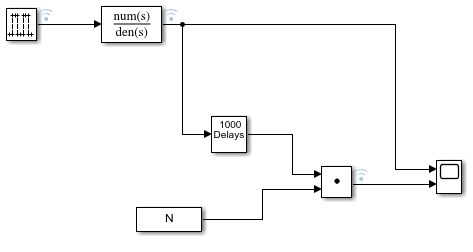
\includegraphics[scale=0.9]{Q3cblocks.PNG}
        \caption{\label{fig:q3cblocks}Simulink model to generate the low pass filter and transversal filter.}
    \end{figure}
    
    \begin{figure}[H]
    \centering
        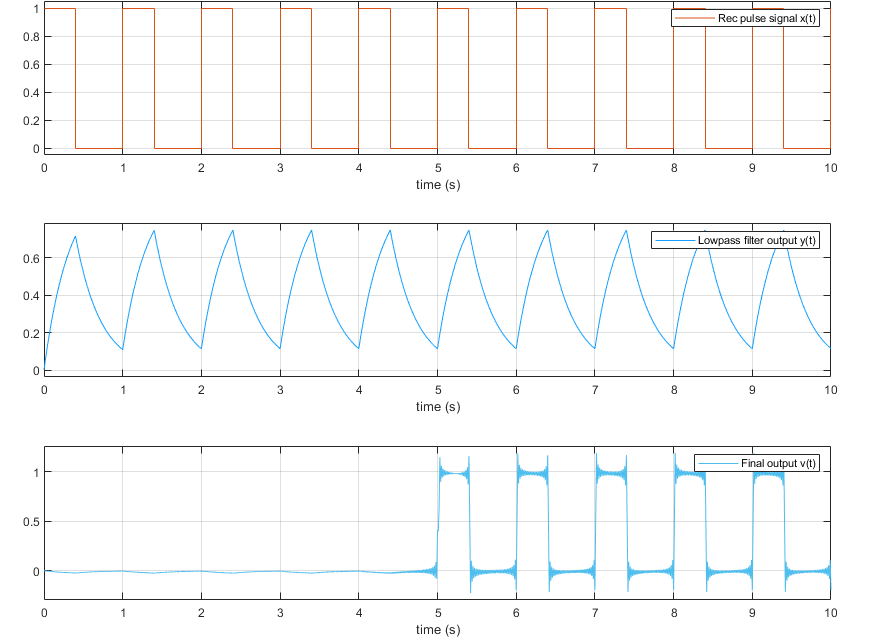
\includegraphics[scale=0.7]{Q3c.png}
        \caption{\label{fig:q3csignals}Signal waveforms of $x(t)$, $y(t)$ and $v(t)$.}
    \end{figure}


\end{enumerate}


\newpage
\section*{Appendix}
\subsection*{MATLAB Code}

%\begin{verbatim}
%%%%%%%%%%%%%%%% this code listing style maybe a little bit easier to read %%%%%%

1. Codes for Question 1 
 \begin{lstlisting}[frame=single]
%% Input Signal
% Part b), evaluating the occupied bandwidth W

% Initialisation
P = [];
n = 0;
Pt = 0.4; % Power of one period of x(t) in time domain
sum = power(n); % Starting the summation with power of x[0]
fprintf("Currently n=%2d, the power sums to: %.4f\n",n,sum)

% Summing the power spectra
while sum <= (0.98*Pt)
    n = n+1;
    P(n) = power(n);
    sum = sum + 2*P(n);
    fprintf("Currently n=%2d, the power sums to: %.4f\n",n,sum);
end

% Bandwidth
W = length(P);
fprintf('The occupied bandwidth, W = %gHz.\n',W);

%% Channel Equalisation
% Part b), graphing the signal after passing through LPF

% Initialisation
X_orig = [];
Ch_out = [];

% Calculating the channel output
for n = 0:14
    X_orig(n+1) = Xf(n);
    Ch_out(n+1) = Xf(n)*Hf(n);
end

% Plotting original signal and signal after passing through LPF
n = [0:14];
figure(1);
set(gcf,'color','w');

subplot(2,1,1) % Amplitude Plot
stem(n, abs(X_orig))
hold on
stem(n, abs(Ch_out))
hold off
title("Amplitude of X(f) and X(f)\cdotH(f)");
xlabel("Frequency (Hz)")
ylabel("Amplitude")
legend("X(f)","X(f)\cdotH(f)")

subplot(2,1,2) % Phase Plot
stem(n, angle(X_orig))
hold on
stem(n, angle(Ch_out))
hold off
title("Phase of X(f) and X(f)\cdotH(f)");
xlabel("Frequency (Hz)")
ylabel("Phase (rad)")
legend("X(f)","X(f)\cdotH(f)")

%% Functions
% Power Function
function P = power(n)
    % Constants 
    T0 = 1;
    tau = 0.4;
    c = tau/T0;
    
    % Power for x[n]
    P = (c*sinc(n*c))^2;
end

% Fourier Transform of x(t)
function X = Xf(n)
    % Constants 
    T0 = 1;
    tau = 0.4;
    c = tau/T0;
    
    % Transfer function
    X = c*sinc(n*c);
end
\end{lstlisting}
2. Codes for Question 3 (c)
\begin{lstlisting}[frame=single]
numofdelay=1000;
n1=-numofdelay/2:1:-1;
n2=1:1:numofdelay/2;
N=[-(100./(pi*n1)).*(-1).^(n1),1,-(100./(pi*n2)).*(-1).^(n2)];
\end{lstlisting}

%\end{verbatim}

\end{document}
